% !TEX TS-program = pdflatexmk

\documentclass[14pt]{beamer}
\usepackage{newtxtext,newtxmath}
\usepackage{microtype}
\usepackage[english]{babel}
\usepackage{hyperref}
\usepackage{graphicx}
\usepackage{listings}
\lstloadlanguages{Python}
\lstset{language=Python}
\lstset{%
basicstyle=\ttfamily\bfseries,
keywordstyle=\color{blue}, emph={self}, emphstyle={\color{blue}},
identifierstyle=,
commentstyle=\color{brown},
stringstyle=\color{green!50!black},
showstringspaces=false,
emphstyle={[2]\color{purple}},
}
\usepackage{tikz}
\usepackage{pgfplots}
\usepackage{forest}
\usetikzlibrary{calc}
\usetikzlibrary{shapes}
\usetikzlibrary{positioning}
\usetikzlibrary{arrows}
\usepackage{array}
\newcolumntype{L}[1]{>{\raggedright\let\newline\\\arraybackslash\hspace{0pt}}m{#1}}

\mode<presentation>{
\usetheme{Madrid}
\definecolor{uabgreen}{cmyk}{.89,.31,.78,.17}
\usecolortheme[named=uabgreen]{structure}
\setbeamertemplate{navigation symbols}{}
\setbeamertemplate{footline}[frame number]
\setbeamertemplate{section in toc}[square]
\setbeamertemplate{subsection in toc}[square]
\setbeamertemplate{items}[square]
\setbeamercovered{transparent=5}
}

\newcommand{\keyword}[1]{{\color{blue}#1}}
\newcommand{\cmnt}[1]{{\color{gray}#1}}
\newcommand{\str}[1]{{\color{green!50!black}#1}}
\newcommand{\num}[1]{{\color{green!55!blue}#1}}
\newcommand{\defn}[1]{{\color{purple}#1}}

\newcommand{\limpl}{\Rightarrow}
\newcommand{\liff}{\Leftrightarrow}

\newcommand{\tab}{\hspace{1em}}

\author[Dr. Bethard]{Dr. Steven Bethard}
\institute[UAB CIS]{%
Computer and Information Sciences\\
University of Alabama at Birmingham}

\AtBeginSection[]
{
  \begin{frame}<beamer>{Outline}
    \tableofcontents[currentsection]
  \end{frame}
}

\tikzset{
  invisible/.style={opacity=0,text opacity=0},
  text visible on/.code={%
    \alt<#1>{}{\pgfkeysalso{text opacity=0}}
  },
  visible on/.code={%
    \alt<#1>{}{\pgfkeysalso{invisible}}
  },
  filled on/.code={%
    \alt<#1>{\pgfkeysalso{fill=gray}}{}
  },
  alt/.code n args={3}{%
    \alt<#1>{\pgfkeysalso{#2}}{\pgfkeysalso{#3}}
  },
}
\forestset{
  edge weight/.style={
    edge label={node[midway,above,sloped]{#1}}},
  invisible/.style={
    /tikz/invisible,
    edge={/tikz/invisible}},
  visible on filled on/.code n args={2}{%
    \alt<#1>{\alt<#2>{\pgfkeysalso{fill=gray}}{}}{\pgfkeysalso{invisible}}
  },
  visible on/.code={%
    \alt<#1>{}{\pgfkeysalso{invisible}}
  },
}

\newlength{\wumpusgridsize}
\newenvironment{wumpusgrid}[2]{%
\setlength{\wumpusgridsize}{#2}
\begin{tikzpicture}
\draw[very thick,step=\wumpusgridsize] (0,0) grid (#1\wumpusgridsize, #1\wumpusgridsize);
}{%
\end{tikzpicture}
}
\newcommand{\wumpustop}[5][]{%
\only<#2>{\node[#1] at (#3\wumpusgridsize+0.5\wumpusgridsize,#4\wumpusgridsize+0.75\wumpusgridsize) {#5};}
}
\newcommand{\wumpusbottom}[5][]{%
\only<#2>{\node[#1] at (#3\wumpusgridsize+0.5\wumpusgridsize,#4\wumpusgridsize+0.25\wumpusgridsize) {#5};}
}
\newcommand{\wumpusagent}[3]{\wumpusbottom{#1}{#2}{#3}{\fbox{A}}}
\newcommand{\wumpuspercept}[4]{%
\only<#1>{\node[red,inner sep=0pt] at (#2\wumpusgridsize+0.25\wumpusgridsize,#3\wumpusgridsize+0.75\wumpusgridsize) {\textbf{#4}};}
}
\newcommand{\wumpusknowledge}[4]{%
\only<#1>{\node[draw,cloud,inner sep=0pt,text width=1em,align=center] at (#2\wumpusgridsize+0.75\wumpusgridsize,#3\wumpusgridsize+0.75\wumpusgridsize) {\footnotesize #4};}
}


\newcommand{\bxcyalignment}{
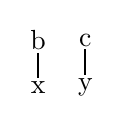
\begin{tikzpicture}[baseline=-0.25em,inner sep=0.1em]
  \node (b) at (-0.3,0.3) {b};
  \node (c) at (0.3,0.3)  {c};
  \node (x) at (-0.3,-0.3)  {x};
  \node (y) at (0.3,-0.3) {y};
  \draw[thick] (b) -- (x);
  \draw[thick] (c) -- (y);
\end{tikzpicture}
}
\newcommand{\bycxalignment}{
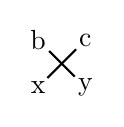
\begin{tikzpicture}[baseline=-0.25em,inner sep=0.1em]
  \node (b) at (-0.3,0.3) {b};
  \node (c) at (0.3,0.3)  {c};
  \node (x) at (-0.3,-0.3)  {x};
  \node (y) at (0.3,-0.3) {y};
  \draw[thick] (b) -- (y);
  \draw[thick] (c) -- (x);
\end{tikzpicture}
}
\newcommand{\byalignment}{
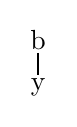
\begin{tikzpicture}[baseline=-0.25em,inner sep=0.1em]
  \node (b) at (0,0.3) {b};
  \node (y) at (0,-0.3) {y};
  \draw[thick] (b) -- (y);
\end{tikzpicture}
}


\title{Learning Probabilistic Models}
\date[]{9 Apr 2015}

\begin{document}

\begin{frame}
\titlepage
\end{frame}

\begin{frame}{Outline}
\tableofcontents
\end{frame}

\section{Naive Bayes}

\subsection{Models}

\begin{frame}{Naive Bayes Networks}
\begin{columns}[t]
\begin{column}{2in}
\begin{block}{Bayesian Network}
Represents all variable dependence relations
\end{block}
\begin{center}
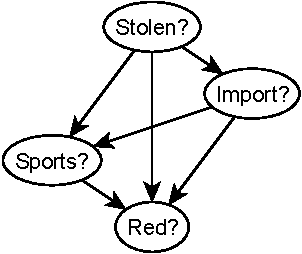
\includegraphics[scale=.75]{stolen-bayes-net}
\end{center}
\end{column}
\pause
\begin{column}{2in}
\begin{block}{Naive Bayes Network}
Assumes features are conditionally independent given the class variable
\end{block}
\begin{center}
\includegraphics[scale=.75]{stolen-naive-bayes}
\end{center}
\end{column}
\end{columns}
\end{frame}

\begin{frame}{Naive Bayes Models}
\begin{block}{Given class $C$ and features $F_1,\ldots,F_n$}
$
\begin{array}{llll}
\lefteqn{\mathbf{P}(C|F_1,F_2,\ldots,F_n)} \\
& = & \pause\alpha\mathbf{P}(F_1,F_2,\ldots,F_n|C)\mathbf{P}(C) & \mbox{Bayes' Rule} \\
& = & \pause\alpha\mathbf{P}(F_1|C)\mathbf{P}(F_2|C)\ldots\mathbf{P}(F_n|C)\mathbf{P}(C) & \mbox{Naive Bayes}
\end{array}
$
\end{block}
\pause
\vspace{-1pt}
\begin{block}{Naive Bayes models}
$\mathbf{P}(C|F_1,F_2,\ldots,F_n) = \alpha\mathbf{P}(C)\prod\limits_{i=1}^{n}\mathbf{P}(F_{i}|C)$
\end{block}
\pause
\vspace{-1pt}
\begin{block}{Training models}
\begin{itemize}
\item Find the probability of each class
\item Find the probability of each feature given the class
\end{itemize}
\end{block}
\end{frame}

\subsection{Examples}

\begin{frame}{Naive Bayes Classification}
\centering
\begin{tabular}[t]{lll|l}
Origin?  & Color? & Type?  & Stolen? \\
\hline
import   & red    & sports & yes \\
import   & red    & sports & yes \\
domestic & white  & sports & yes \\
domestic & red    & van    & yes \\
import   & red    & van    & no \\
domestic & white  & sports & no \\
\end{tabular}

\pause
\begin{block}{A domestic red sports car}
\small
$
\begin{array}{@{}l@{\hspace{.1em}}l@{\hspace{.1em}}l@{\hspace{.1em}}l@{\hspace{.1em}}l@{\hspace{.1em}}l@{\hspace{.1em}}l@{}}
\pause
P(y|d,r,s) & = & \pause\alpha P(y)P(d|y)P(r|y)P(s|y) 
           & = & \pause\alpha\cdot\pause\frac{2}{3}\cdot\pause\frac{1}{2}\cdot\pause\frac{3}{4}\cdot\pause\frac{3}{4}
           & = & \pause\frac{3}{16}\alpha
\\
\pause
P(n|d,r,s) & = & \pause\alpha P(n)P(d|n)P(r|n)P(s|n)
           & = & \pause\alpha\cdot\frac{1}{3}\cdot\frac{1}{2}\cdot\frac{1}{2}\cdot\frac{1}{2}
           & = & \pause\frac{1}{24}\alpha
\end{array}
$
\normalsize
\medskip

\pause
Predict stolen?
\pause
\alert{yes}
\hfill
\pause
At what probability?
\pause
$\alert{\frac{9}{11}} = \frac{\frac{3}{16}}{\frac{3}{16} + \frac{1}{24}}$
\end{block}
\end{frame}

\begin{frame}{Naive Bayes Exercise}
\centering
\begin{tabular}[t]{cc|c}
Ends with -ed  & Initial Capital  & Part of Speech \\
\hline
no             & no               & noun \\
no             & yes              & noun \\
no             & yes              & noun \\
yes            & no               & noun \\
yes            & yes              & noun \\
no             & no               & verb \\
yes            & no               & verb \\
yes            & yes              & verb \\
\end{tabular}\\
\bigskip
Assign part of speech tags:
\tab\tab
\begin{tabular}[t]{cc}
John            & tripped \\
\visible<2->{
noun            & verb    \\
$\frac{27}{32}$ & $\frac{5}{8}$
%.84375          & .625 \\
}
\end{tabular}
% John
% P(POS=n | ED=n , CAP=y)
% = \alpha P(POS=n) P(ED=n | POS=n) P(CAP=y | POS=n)
% = \alpha \frac{5}{8} \cdot \frac{3}{5} \cdot \frac{3}{5}
% = \alpha \frac{9}{40}
% P(POS=v | ED=n , CAP=y)
% = \alpha P(POS=v) P(ED=n | POS=v) P(CAP=y | POS=v)
% = \alpha \frac{3}{8} \cdot \frac{1}{3} \cdot \frac{1}{3}
% = \alpha \frac{1}{24}
% \alpha = \frac{15}{4}
% P(POS | ED=n , CAP=y) = \langle \frac{27}{32}, \frac{5}{32} \rangle
% tripped
% P(POS=n | ED=y , CAP=n)
% = \alpha P(POS=n) P(ED=y | POS=n) P(CAP=n | POS=n)
% = \alpha \frac{5}{8} \cdot \frac{2}{5} \cdot \frac{2}{5}
% = \alpha \frac{1}{10}
% P(POS=v | ED=y , CAP=n)
% = \alpha P(POS=v) P(ED=y | POS=v) P(CAP=n | POS=v)
% = \alpha \frac{3}{8} \cdot \frac{2}{3} \cdot \frac{2}{3}
% = \alpha \frac{1}{6}
% \alpha = \frac{15}{4}
% P(POS | ED=y , CAP=n) = \langle \frac{3}{8}, \frac{5}{8} \rangle
\end{frame}

\subsection{Properties}

\begin{frame}{Naive Bayes Properties}
\begin{block}{Naive Bayes assumption is hardly ever true}
\begin{itemize}
\item Probability estimates of Naive Bayes are poor
\item Classification decisions are often surprisingly good
\end{itemize}
\end{block}
\pause
\begin{block}{Empirical Observations}
\begin{itemize}
\item Works best when many equally important features
\item Somewhat robust to noise (uninformative) features
\item Training and classification are typically fast
\end{itemize}
\end{block}
\end{frame}

\section{Expectation Maximization}

\subsection{Hidden Variables}

\begin{frame}{A Coin Example}
\thickmuskip=1mu
Given two coins:
\begin{description}[A]
\item[A] with $P(A=H)$ for heads and $P(A=T)$ for tails
\item[B] with $P(B=H)$ for heads and $P(B=T)$ for tails
\end{description}
\bigskip
Estimate $\mathbf{P}(A)$ and $\mathbf{P}(B)$ from the coin tosses:\\
\smallskip
\begin{tabular}{ @{} c c c c c c }
& & \visible<2->{$A=H$ & $A=T$ & $B=H$ & $B=T$} \\
A & \tt HHHHTHHHHH \visible<2->{& 9 & 1 & &} \\
B & \tt HTHTTTHHTT \visible<2->{& & & 4 & 6} \\
A & \tt HTHHHHHTHH \visible<2->{& 8 & 2 & &} \\
A & \tt THHHTHHHTH \visible<2->{& 7 & 3 & &} \\
B & \tt HTTTHHTHTH \visible<2->{& & & 5 & 5} \\
\end{tabular}\\
\medskip
\visible<3->{
$\begin{array}{ c c }
\mathbf{P}(A) = \left\langle \frac{24}{24 + 6}, \frac{6}{24 + 6} \right\rangle
& \mathbf{P}(B) = \left\langle \frac{9}{9 + 11}, \frac{11}{9 + 11} \right\rangle
\end{array}$}
\end{frame}

\begin{frame}{A Coin Example with a Hidden Variable}
\thickmuskip=1mu
But what if we didn't know which coin was being tossed?
\begin{itemize}
\item i.e. $P(C=A)$ and $P(C=B)$ are unknown
\end{itemize}
\medskip
Estimate $\mathbf{P}(A)$, $\mathbf{P}(B)$ from the coin tosses:\\
\smallskip
\begin{tabular}{ @{} c c c c c c c }
\visible<3->{$C=A$ & $C=B$} & & $A=H$ & $A=T$ & $B=H$ & $B=T$ \\
\only<3->{0.80} & \alt<3->{0.20}{?} & \tt HHHHTHHHHH & \only<4->{7.2} & \only<5->{0.8} & \only<6->{1.8 & 0.2} \\
\only<3->{0.35} & \alt<3->{0.65}{?} & \tt HTHTTTHHTT & \only<7->{1.4 & 2.1} & \only<8->{2.6 & 3.9} \\
\only<3->{0.73} & \alt<3->{0.27}{?} & \tt HTHHHHHTHH & \only<9->{5.8 & 1.5 & 2.2 & 0.5} \\
\only<3->{0.65} & \alt<3->{0.35}{?} & \tt THHHTHHHTH & \only<9->{4.5 & 1.9 & 2.5 & 1.1} \\
\only<3->{0.45} & \alt<3->{0.55}{?} & \tt HTTTHHTHTH & \only<9->{2.2 & 2.2 & 2.8 & 2.8} \\
\end{tabular}\\
\medskip
\visible<2->{
What if we knew $\mathbf{P}(C|\texttt{HHHHTHHHHH})$, etc.?}\\
\smallskip
\visible<10->{
$\begin{array}{ c c }
\mathbf{P}(A) = \left\langle \frac{21.3}{21.3 + 8.6}, \frac{8.6}{21.3 + 8.6} \right\rangle
& \mathbf{P}(B) = \left\langle \frac{11.7}{11.7 + 8.4}, \frac{8.4}{11.7 + 8.4} \right\rangle
\end{array}$}
\end{frame}

\begin{frame}{Probability of the Hidden Variable}
\thickmuskip=1mu
$\begin{array}{ l }
P(C=A|\texttt{HHHHTHHHHH}) \\
\pause
= \alpha P(\texttt{HHHHTHHHHH}|C=A) P(C=A) \\
\pause
= \alpha P(\texttt{H}|C=A) P(\texttt{H}|C=A) \ldots P(\texttt{H}|C=A) P(C=A) \\
\pause
= \alpha P(\texttt{H}|A) P(\texttt{H}|A) \ldots P(\texttt{H}|A) P(C=A) \\
\end{array}$\\
\bigskip
\pause
Say we make an initial guess:
\begin{itemize}
\item $\mathbf{P}(C) = \left\langle 0.5, 0.5\right\rangle$
\item $\mathbf{P}(A) = \left\langle 0.6, 0.4\right\rangle$
\item $\mathbf{P}(B) = \left\langle 0.5, 0.5\right\rangle$
\end{itemize}
Then:\\
$P(C=A|\texttt{HHHHTHHHHH}) = \pause \alpha \cdot 0.6^{9} \cdot 0.4^{1} \cdot 0.5 \approx .00202 \alpha$ \\
\pause
$P(C=B|\texttt{HHHHTHHHHH}) = \alpha \cdot 0.5^{9} \cdot 0.5^{1} \cdot 0.5 \approx .00049 \alpha$ \\
\pause
$\mathbf{P}(C|\texttt{HHHHTHHHHH}) \approx \left\langle .80, .20 \right\rangle$
\end{frame}

\subsection{Algorithm}

\begin{frame}{The Expectation Maximization Algorithm}
\begin{enumerate}
\item Make initial guess of all probabilities $\mathbf{P}(X_0), \mathbf{P}(X_1), \ldots$
\item\label{item:calculate-hidden} Calculate $\mathbf{P}(X_h|\text{data})$ for all hidden variables $X_h$
\item Tabulate partial counts for $X_0, X_1, \ldots$ from data
\item Normalize partial counts to get $\mathbf{P}(X_0), \mathbf{P}(X_1), \ldots$
\item Goto \ref{item:calculate-hidden}
\end{enumerate}
\end{frame}

\begin{frame}{EM in Machine Translation}
Given parallel sentences
\begin{itemize}
\item $b c \Leftrightarrow x y$
\item $b \Leftrightarrow y$
\end{itemize}
\visible<2->{
Make initial guess of all probabilities
\begin{itemize}
\thickmuskip=1mu
\item $P(b=x) = \frac{1}{2}$, $P(b=y) = \frac{1}{2}$, $P(c=x) = \frac{1}{2}$, $P(c=y) = \frac{1}{2}$
\end{itemize}
}
\visible<3->{
Calculate $\mathbf{P}(A|\text{data})$ for alignments $A$ in $b c \Leftrightarrow x y$:
\begin{itemize}
\item
$P\left(\text{\bxcyalignment} \Bigm | b c \Leftrightarrow x y \right)
= \alpha \cdot \visible<4->{\frac{1}{2} \cdot \frac{1}{2} \visible<5->{= \frac{1}{4} \alpha \visible<7->{\Rightarrow \frac{1}{2}}}}$
\item
$P\left(\text{\bycxalignment} \Bigm | b c \Leftrightarrow x y \right)
= \alpha \cdot \visible<6->{\frac{1}{2} \cdot \frac{1}{2} \visible<6->{= \frac{1}{4} \alpha \visible<7->{\Rightarrow \frac{1}{2}}}}$
\end{itemize}
}
\visible<8->{
Calculate $\mathbf{P}(A|\text{data})$ for alignments $A$ in $b \Leftrightarrow y$:
\begin{itemize}
\item
$P\left(\text{\byalignment} \Bigm | b \Leftrightarrow y \right)
= \alpha \cdot \visible<9->{\frac{1}{2} \visible<10->{\Rightarrow 1}}$
\end{itemize}
}
\end{frame}

\begin{frame}{EM in Machine Translation}
\setbeamercovered{invisible}
\renewcommand{\arraystretch}{1.2}
Tabulate partial counts from $b c \Leftrightarrow x y$ alignments:
\begin{itemize}
\item $P\left(\text{\bxcyalignment} \Bigm | bc \Leftrightarrow xy \right) \Rightarrow
\pause
\begin{array} { l l l }
\#(b=x) & \mathrel{+}= & \frac{1}{2} \\
\#(c=y) & \mathrel{+}= & \frac{1}{2} \\
\end{array}$
\pause
\item $P\left(\text{\bycxalignment} \Bigm | bc \Leftrightarrow xy \right) \Rightarrow
\pause
\begin{array} { l l l }
\#(b=y) & \mathrel{+}= & \frac{1}{2} \\
\#(c=x) & \mathrel{+}= & \frac{1}{2} \\
\end{array}$
\end{itemize}
\pause
Tabulate partial counts from $b \Leftrightarrow y$ alignments:
\begin{itemize}
\item $P\left(\text{\byalignment} \Bigm | b \Leftrightarrow y \right) \hspace{2.2em} \Rightarrow
\pause
\begin{array}{ l l l }
\#(b=y) & \mathrel{+}= & 1
\end{array}$
\end{itemize}
\pause
Normalize partial counts to get new probabilities:
\begin{itemize}
\thickmuskip=1mu
\item $\mathbf{P}(b)$:
$P(b=x) = \pause\frac{\frac{1}{2}}{\frac{1}{2} + \frac{3}{2}} = \frac{1}{4}$
\pause,
$P(b=y) = \pause\frac{\frac{3}{2}}{\frac{1}{2} + \frac{3}{2}} = \frac{3}{4}$
\pause
\item $\mathbf{P}(c)$:
$P(c=x) = \pause\frac{\frac{1}{2}}{\frac{1}{2} + \frac{1}{2}} = \frac{1}{2}$
\pause,
$P(c=y) = \pause\frac{\frac{1}{2}}{\frac{1}{2} + \frac{1}{2}} = \frac{1}{2}$
\end{itemize}
\end{frame}

\begin{frame}{EM in Machine Translation Exercise}
Given sentences:
\begin{itemize}
\item $b c \Leftrightarrow x y$
\item $b \Leftrightarrow y$
\end{itemize}
With possible alignments:\\
\begin{tabular}{ @{\hspace{1em}} c c @{\hspace{2em}} c }
\multicolumn{2}{ @{\hspace{1em}} c @{\hspace{2em}} }{$b c \Leftrightarrow x y$} & $b \Leftrightarrow y$ \\
\bxcyalignment & \bycxalignment & \byalignment
\end{tabular}\\
\smallskip
And current probabilities:
\begin{itemize}
\thickmuskip=1mu
\item
$P(b=x) = \frac{1}{4}$,
$P(b=y) = \frac{3}{4}$,
$P(c=x) = \frac{1}{2}$,
$P(c=y) = \frac{1}{2}$
\end{itemize}
Calculate the probabilities after the next iteration of EM
\visible<2->{
\begin{itemize}
\thickmuskip=1mu
\item
$P(b=x) = \frac{1}{8}$,
$P(b=y) = \frac{7}{8}$,
$P(c=x) = \frac{3}{4}$,
$P(c=y) = \frac{1}{4}$
\end{itemize}
}
\end{frame}

\subsection{Properties}

\begin{frame}{Expectation Maximization Properties}
Theoretical:
\begin{itemize}
\item Each iteration increases the log likelihood of the data
\item Often guaranteed to converge to a local maximum
\item Hill climbing, but no step size needed
\end{itemize}
\bigskip
\pause
Practical:
\begin{itemize}
\item Initialization can be critical
\item May overfit to noise in the data
\end{itemize}
\end{frame}

\part{Key Ideas}
\begin{frame}{Key Ideas}
\begin{block}{Naive Bayes}
\begin{itemize}
\item Assume features conditionally independent given class
\item Maximum likelihood estimates (i.e. count and divide)
\end{itemize}
\end{block}
\begin{block}{Expectation Maximization}
\begin{itemize}
\item Guess probabilities for all variables in model
\item Calculate probabilities of hidden variables given data
\item Tabulate partial counts $\Rightarrow$ new variable probabilities
\item Iterate until local maximum is reached
\end{itemize}
\end{block}
\end{frame}

\end{document}


